
\documentclass[letterpaper,hide notes,xcolor={table,svgnames},pdftex,10pt]{beamer}
\def\showexamples{t}

\usecolortheme{crane}
\setbeamertemplate{navigation symbols}{}

\usetheme{MyPittsburgh}
\usepackage{hyperref}
\usepackage{graphicx,xspace}
\usepackage[normalem]{ulem}
\usepackage{multicol}
\usepackage{amsmath,amssymb,amsthm,graphicx,xspace}
\newcommand\SF[1]{$\bigstar$\footnote{SF: #1}}

\usepackage[sfdefault,lf]{carlito}
\usepackage[T1]{fontenc}
\usepackage[scaled]{beramono}
\usepackage{tikzpagenodes}
\newcommand{\Rplus}{\protect\hspace{-.1em}\protect\raisebox{.35ex}{\small{\small\textbf{+}}}}
\newcommand{\Cpp}{\mbox{C\Rplus\Rplus}\xspace}

\newcounter{tmpnumSlide}
\newcounter{tmpnumNote}

\newcommand\mnote[1]{%
	\addtocounter{tmpnumSlide}{1}
	\ifdefined\showcues {~\tiny\fbox{\arabic{tmpnumSlide}}}\fi
	\note{\setlength{\parskip}{1ex}\addtocounter{tmpnumNote}{1}\textbf{\Large \arabic{tmpnumNote}:} {#1\par}}}

\newcommand\mmnote[1]{\note{\setlength{\parskip}{1ex}#1\par}}


\newcommand\mquestion[2]{{~\color{red}\fbox{?}}\note{\setlength{\parskip}{1ex}\par{\Large \textbf{?}} #1} \note{\setlength{\parskip}{1ex}\par{\Large \textbf{A}} #2\par}\ifdefined \presentationonly \pause \fi}

\newcommand\blackboard[1]{%
	\ifdefined   \showblackboard
		{#1}
	\else {\begin{center} \fbox{\colorbox{blue!30}{%
						\begin{minipage}{.95\linewidth}%
							\hspace{\stretch{1}} Some space intentionally left blank; done at the blackboard.%
						\end{minipage}}}\end{center}}%
	\fi%
}

\usepackage{listings}
\lstset{%
	keywordstyle=\bfseries,
	aboveskip=15pt,
	belowskip=15pt,
	captionpos=b,
	identifierstyle=\ttfamily,
	frame=lines,
	numbers=left, basicstyle=\scriptsize, numberstyle=\tiny, stepnumber=0, numbersep=2pt}

\usepackage{siunitx}
\newcommand\sius[1]{\num[group-separator = {,}]{#1}\si{\micro\second}}
\newcommand\sims[1]{\num[group-separator = {,}]{#1}\si{\milli\second}}
\newcommand\sins[1]{\num[group-separator = {,}]{#1}\si{\nano\second}}
\sisetup{group-separator = {,}, group-digits = true}

%% -------------------- tikz --------------------
\usepackage{tikz}
\usetikzlibrary{positioning}
\usetikzlibrary{arrows,backgrounds,automata,decorations.shapes,decorations.pathmorphing,decorations.markings,decorations.text}

\tikzstyle{place}=[circle,draw=blue!50,fill=blue!20,thick, inner sep=0pt,minimum size=6mm]
\tikzstyle{transition}=[rectangle,draw=black!50,fill=black!20,thick, inner sep=0pt,minimum size=4mm]

\tikzstyle{block}=[rectangle,draw=black, thick, inner sep=5pt]
\tikzstyle{bullet}=[circle,draw=black, fill=black, thin, inner sep=2pt]

\tikzstyle{pre}=[<-,shorten <=1pt,>=stealth',semithick]
\tikzstyle{post}=[->,shorten >=1pt,>=stealth',semithick]
\tikzstyle{bi}=[<->,shorten >=1pt,shorten <=1pt, >=stealth',semithick]

\tikzstyle{mut}=[-,>=stealth',semithick]

\tikzstyle{treereset}=[dashed,->, shorten >=1pt,>=stealth',thin]

\usepackage{ifmtarg}
\usepackage{xifthen}
\makeatletter
% new counter to now which frame it is within the sequence
\newcounter{multiframecounter}
% initialize buffer for previously used frame title
\gdef\lastframetitle{\textit{undefined}}
% new environment for a multi-frame
\newenvironment{multiframe}[1][]{%
	\ifthenelse{\isempty{#1}}{%
		% if no frame title was set via optional parameter,
		% only increase sequence counter by 1
		\addtocounter{multiframecounter}{1}%
	}{%
		% new frame title has been provided, thus
		% reset sequence counter to 1 and buffer frame title for later use
		\setcounter{multiframecounter}{1}%
		\gdef\lastframetitle{#1}%
	}%
	% start conventional frame environment and
	% automatically set frame title followed by sequence counter
	\begin{frame}%
		\frametitle{\lastframetitle~{\normalfont(\arabic{multiframecounter})}}%
		}{%
	\end{frame}%
}
\makeatother

\makeatletter
\newdimen\tu@tmpa%
\newdimen\ydiffl%
\newdimen\xdiffl%
\newcommand\ydiff[2]{%
	\coordinate (tmpnamea) at (#1);%
	\coordinate (tmpnameb) at (#2);%
	\pgfextracty{\tu@tmpa}{\pgfpointanchor{tmpnamea}{center}}%
	\pgfextracty{\ydiffl}{\pgfpointanchor{tmpnameb}{center}}%
	\advance\ydiffl by -\tu@tmpa%
}
\newcommand\xdiff[2]{%
	\coordinate (tmpnamea) at (#1);%
	\coordinate (tmpnameb) at (#2);%
	\pgfextractx{\tu@tmpa}{\pgfpointanchor{tmpnamea}{center}}%
	\pgfextractx{\xdiffl}{\pgfpointanchor{tmpnameb}{center}}%
	\advance\xdiffl by -\tu@tmpa%
}
\makeatother
\newcommand{\copyrightbox}[3][r]{%
	\begin{tikzpicture}%
		\node[inner sep=0pt,minimum size=2em](ciimage){#2};
		\usefont{OT1}{phv}{n}{n}\fontsize{4}{4}\selectfont
		\ydiff{ciimage.south}{ciimage.north}
		\xdiff{ciimage.west}{ciimage.east}
		\ifthenelse{\equal{#1}{r}}{%
			\node[inner sep=0pt,right=1ex of ciimage.south east,anchor=north west,rotate=90]%
			{\raggedleft\color{black!50}\parbox{\the\ydiffl}{\raggedright{}#3}};%
		}{%
			\ifthenelse{\equal{#1}{l}}{%
				\node[inner sep=0pt,right=1ex of ciimage.south west,anchor=south west,rotate=90]%
				{\raggedleft\color{black!50}\parbox{\the\ydiffl}{\raggedright{}#3}};%
			}{%
				\node[inner sep=0pt,below=1ex of ciimage.south west,anchor=north west]%
				{\raggedleft\color{black!50}\parbox{\the\xdiffl}{\raggedright{}#3}};%
			}
		}
	\end{tikzpicture}
}


%% --------------------

%\usepackage[excludeor]{everyhook}
%\PushPreHook{par}{\setbox0=\lastbox\llap{MUH}}\box0}

%\vspace*{\stretch{1}

%\setbox0=\lastbox \llap{\textbullet\enskip}\box0}

\setlength{\parskip}{\fill}

\newcommand\noskips{\setlength{\parskip}{1ex}}
\newcommand\doskips{\setlength{\parskip}{\fill}}

\newcommand\xx{\par\vspace*{\stretch{1}}\par}
\newcommand\xxs{\par\vspace*{2ex}\par}
\newcommand\tuple[1]{\langle #1 \rangle}
\newcommand\code[1]{{\sf \footnotesize #1}}
\newcommand\ex[1]{\uline{Example:} \ifdefined \presentationonly \pause \fi
	\ifdefined\showexamples#1\xspace\else{\uline{\hspace*{2cm}}}\fi}

\newcommand\ceil[1]{\lceil #1 \rceil}


\AtBeginSection[]
{
	\begin{frame}
		\frametitle{Outline}
		\tableofcontents[currentsection]
	\end{frame}
}



\pgfdeclarelayer{edgelayer}
\pgfdeclarelayer{nodelayer}
\pgfsetlayers{edgelayer,nodelayer,main}

\tikzstyle{none}=[inner sep=0pt]
\tikzstyle{rn}=[circle,fill=Red,draw=Black,line width=0.8 pt]
\tikzstyle{gn}=[circle,fill=Lime,draw=Black,line width=0.8 pt]
\tikzstyle{yn}=[circle,fill=Yellow,draw=Black,line width=0.8 pt]
\tikzstyle{empty}=[circle,fill=White,draw=Black]
\tikzstyle{bw} = [rectangle, draw, fill=blue!20,
text width=4em, text centered, rounded corners, minimum height=2em]

\newcommand{\CcNote}[1]{% longname
	This work is licensed under the \textit{Creative Commons #1 3.0 License}.%
}
\newcommand{\CcImageBy}[1]{%
	\includegraphics[scale=#1]{creative_commons/cc_by_30.pdf}%
}
\newcommand{\CcImageSa}[1]{%
	\includegraphics[scale=#1]{creative_commons/cc_sa_30.pdf}%
}
\newcommand{\CcImageNc}[1]{%
	\includegraphics[scale=#1]{creative_commons/cc_nc_30.pdf}%
}
\newcommand{\CcGroupBySa}[2]{% zoom, gap
	\CcImageBy{#1}\hspace*{#2}\CcImageNc{#1}\hspace*{#2}\CcImageSa{#1}%
}
\newcommand{\CcLongnameByNcSa}{Attribution-NonCommercial-ShareAlike}

\newenvironment{changemargin}[1]{% 
	\begin{list}{}{% 
		\setlength{\topsep}{0pt}% 
		\setlength{\leftmargin}{#1}% 
		\setlength{\rightmargin}{1em}
		\setlength{\listparindent}{\parindent}% 
		\setlength{\itemindent}{\parindent}% 
		      \setlength{\parsep}{\parskip}% 
		      }% 
		\item[]}{\end{list}}




\title{Lecture 13 --- Concurrency: Synchronization/Atomicity }

\author{Jeff Zarnett \\ \small \texttt{jzarnett@uwaterloo.ca}}
\institute{Department of Electrical and Computer Engineering \\
	University of Waterloo}
\date{\today}


\begin{document}

\begin{frame}
	\titlepage

\end{frame}


\begin{frame}
	\frametitle{Synchronization}

	If a computer only ever did exactly one thing at a time we would have no concurrency and therefore no concurrency (co-ordination) problems.

	A system with multiple processes or multiple threads will have concurrency.

	If the system is multicore, we can have parallelism.

	Either or both of these can lead to various problems.


\end{frame}

\begin{frame}
	\frametitle{Synchronization}

	The author of an application does not decide when a thread runs and when a thread switch will occur.

	These are things the operating system will decide.

	The operating system does not usually give much thought to whether it is a convenient or inconvenient time to run a given thread.


\end{frame}

\begin{frame}
	\frametitle{Synchronization}

	The common English usage of the word ``synchronization'' refers to making two or more things happen at exactly the same time.

	\begin{center}
		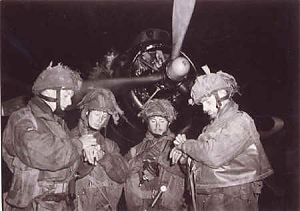
\includegraphics[width=0.4\textwidth]{images/synchronize-watches.jpg}
	\end{center}

	Synchronization in the computer sense is more general:\\
	\quad Some relationship between events: before, during, after.

\end{frame}


\begin{frame}
	\frametitle{Olympic Synchronization}

	\begin{center}
		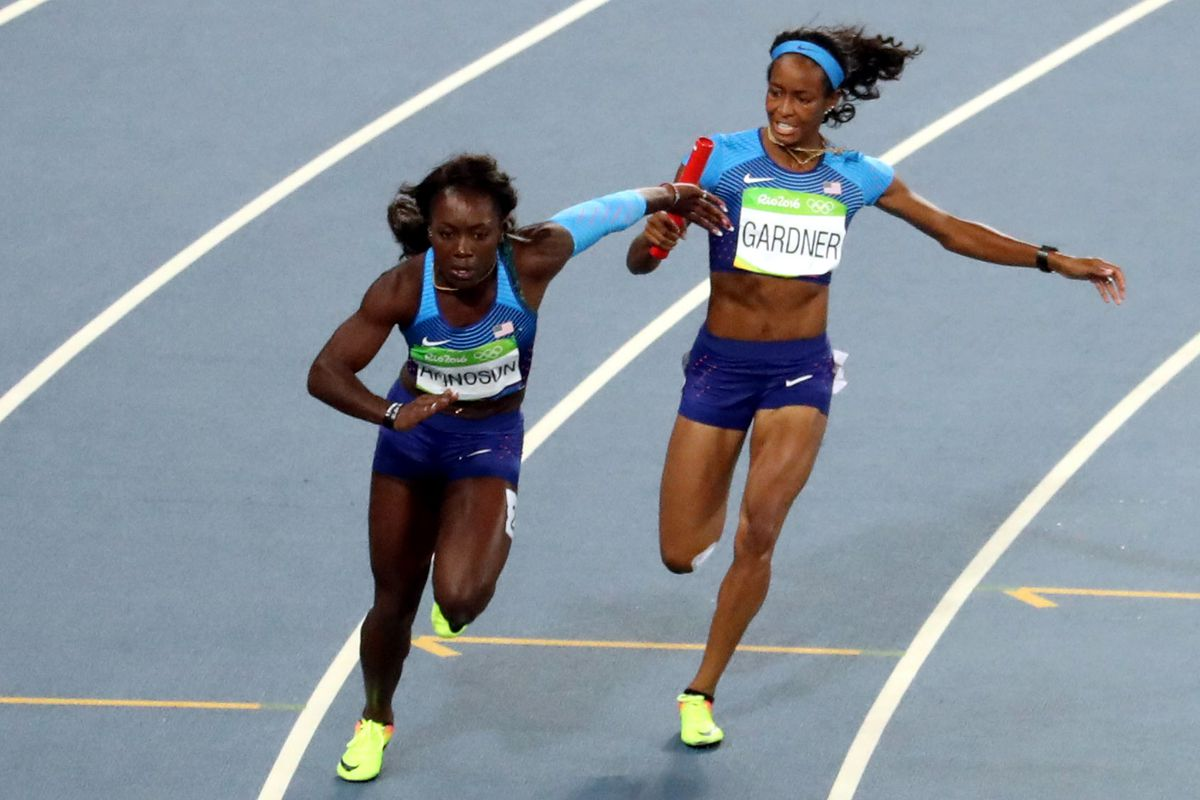
\includegraphics[width=0.5\textwidth]{images/baton-handoff.jpg}
		
\includegraphics[width=0.5\textwidth]{images/skiing.jpg}
	\end{center}

\end{frame}


\begin{frame}
	\frametitle{Serialization}

	\alert{Serialization}: some sort of order of events.

	Certainty that Event $A$ takes place before Event $B$.

	Example: a thread or process that \texttt{wait}s on another.

	Merge sort: the merge thread to wait for the sorting threads to finish.

	Thus the sorting (event $A$) must take place before the merging (event $B$).\\
	\quad Or we could phrase it that $B$ must happen after $A$.


\end{frame}

\begin{frame}
	\frametitle{Mutual Exclusion}

	\alert{Mutual exclusion}: events $C$ and $D$ must not happen at the same time.

	IPC: an area of memory that is shared between two processes.

	If two processes can write to this area, there is some possibility that they both try to access the same place at the same time.

	If we have mutual exclusion, we are certain that $P_{1}$ writing to the shared area (event $C$) does not happen at the same time as $P_{2}$ tries to read it (event $D$).

\end{frame}

\begin{frame}
	\frametitle{Serialization through Messages}

	Suppose we have two people, Alice and Bob\\
	\quad They work at the Springfield Nuclear Power Plant in Sector 7G.

	They work in separate offices and cannot easily see one another.

	Alice works the day shift and Bob works the night shift.

	Due to safety regulations, Alice cannot go home until Bob has arrived.

	This is a situation where we would like serialization: the event of Bob's arrival must take place before the event of Alice's departure.

\end{frame}

\begin{frame}
	\frametitle{Serialization through Messages}

	How can we get such behaviour?

	Simple solution: Alice won't leave until she gets a call from Bob.

	Bob doesn't call until he's arrived at the office.

	This is the sort of thing we do in real life often: ``Text me when you get here''.



\end{frame}

\begin{frame}
	\frametitle{Sequential and Concurrent Events}

	If we are certain that Bob arrives before Alice departs, we can say that these events are \alert{sequential}, because we know the order of events.

	At some point during the workday, Alice ate lunch, and at some point before work, Bob ate lunch.

	But we have no idea who ate lunch first, so we say they ate lunch \alert{concurrently}.

	The formal, strict definition of concurrent is: two events are concurrent if we cannot tell by looking at the program which will happen first.

\end{frame}

\begin{frame}
	\frametitle{Concurrent Events}

	In common parlance, when we say something happened concurrently, it means they happened at the same time (Alice and Bob both had lunch at 12:00).

	Concurrency is not the same as saying that they happened at the exact same time; it's saying that we do not know (and cannot guarantee) an order of events.

	It's possible that Alice had lunch at 12:00 and Bob had lunch at 13:00 or they both ate at 12:00 or Alice had lunch at 13:30 and Bob had lunch at 12:15.

	We do not know.

	The order of concurrent events may change on two runs of the program; this is what we call \alert{nondeterminism}.

\end{frame}

\begin{frame}
	\frametitle{Non-Deterministic Programs}

	In a non-deterministic program, we cannot tell just by looking at the program what the execution order would be.

	If we have two concurrent events: \\
	\quad One in which the program prints ``1'' to the console; and\\
	\quad One in which the program prints ``2'' to the console.

	These could happen in any order.

	So we might see the output as ``12'' or ``21''.

	Which one will happen? Without some form of co-ordination, it could be either.

	If ``12'' is the correct output but ``21'' occurs only very rarely, finding the cause and fixing it might be very painful.


\end{frame}


\begin{frame}
	\frametitle{Heisenbugs}

	This is, what is referred to as a ``Heisenbug''.

	This has nothing to do with the ``Breaking Bad'' TV show.

	\begin{center}
		
\includegraphics[width=0.3\textwidth]{images/heisenberg.jpg}
		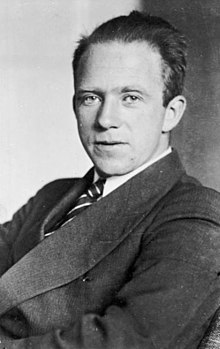
\includegraphics[width=0.1891\textwidth]{images/werner-heisenberg.jpg}
	\end{center}

	It comes from Werner Heisenberg and his scientific principle of uncertainty.

	The Heisenbug is frustrating because the harder we try to track it down, the less likely it is to occur.


\end{frame}


\begin{frame}[fragile]
	\frametitle{Shared Data and Atomic Operations}
	We noted earlier that the need for co-ordination in inter-process communication arises from the fact that some area of memory is shared.

	We also know that all the threads of a process share the same data:.

	Simple example of a shared variable \texttt{x} is manipulated by two threads $A$ and $B$:

	\begin{multicols}{2}
		\textbf{Thread A}
		\begin{verbatim}
	A1. x = 5
	A2. print x
	\end{verbatim}
		\columnbreak
		\textbf{Thread B}
		\begin{verbatim}
	B1. x = 7
	
	\end{verbatim}
	\end{multicols}

\end{frame}

\begin{frame}
	\frametitle{Analyzing the $A$ and $B$ Example}

	This is non-deterministic code.

	There is no co-ordination mechanism here so we cannot say what order these statements will occur.

	Some possible outcomes are:\\
	\quad 5 is printed out and is the final value;\\
	\quad 7 is printed out and is the final value; or\\
	\quad 5 is printed out and 7 is the final value.

	Note that there is no way we can print out 7 and get a final value of 5.


\end{frame}

\begin{frame}
	\frametitle{Interrupts}

	We do not even need multiple threads to have a concurrency problem; just having interrupts in the system is sufficient.

	Consider an application that is used to count occurrences of some event.

	We will store the count in a variable \texttt{count}.

	We will provide some facility for the user to reset the counter (the reset button).

	Each time we detect the event, we increment \texttt{count} with statement of \texttt{count++;} which seems like one single statement.



\end{frame}

\begin{frame}
	\frametitle{Interrupts}

	\texttt{count++;} is broken down into a series of smaller operations.

	If \texttt{count} is 4 and we increment it:

	\begin{enumerate}
		\item Read the current value of \texttt{count} (read 4)
		\item Add 1 to the value (now it's 5)
		\item Write the changed value back to memory (write 5)
	\end{enumerate}


\end{frame}

\begin{frame}
	\frametitle{Interrupts}

	Now imagine an interrupt comes at the worst possible time.

	The interrupt is generated by the reset button: it's supposed to set the value of count to zero.

	\begin{enumerate}
		\item Read the current value of \texttt{count} (read 4)
		\item Add 1 to the value (now it's 5)
		\item INTERRUPT (control goes to the interrupt handler)
		\item Write 0 to the variable (write 0)
		\item END INTERRUPT (control returns to where it was before the interrupt)
		\item Write the changed value back to memory (write 5)
	\end{enumerate}

\end{frame}

\begin{frame}
	\frametitle{Interrupts}

	The variable \texttt{count} shows 5, but it should show 0 (or 1).

	The user pressed the reset button but the count did not reset!

	If the reset interrupt had occurred before reading the variable $\rightarrow$ 1.

	If the reset interrupt had occurred after writing the variable $\rightarrow$ 0.

	The reset action is ``lost''.

\end{frame}

\begin{frame}
	\frametitle{Atomic Operation}

	This problem arises because the instruction \texttt{count++} is really three things (read, add, write) and can be interrupted at any time.

	When we are performing an operation that cannot be interrupted, we say it is \alert{atomic}: indivisible.

	The word stems from Greek word \textit{atomos}, roughly ``not cut-able''.

	Though there are usually some atomic operations available to us in a given system, we cannot be certain that all operations are indivisible.

	In fact, the opposite is likely to be true!

\end{frame}

\begin{frame}
	\frametitle{Atomic Operation}

	Can we get atomic operations with serialization?

	That is, can we make sure that the \texttt{count++} operation completes before the \texttt{count = 0} operation?

	In this case there is no obvious order between the events: the user may press the reset button at any time, even if no event has just occurred.

	Similarly, the event may be detected even if the user is nowhere around and not going to press the reset button.

	Our concept of serialization requires that there exists a correct order:\\
	\quad First this, then that.


\end{frame}


\begin{frame}
	\frametitle{Keep Calm...}

	\begin{center}
		
\includegraphics[width=0.4\textwidth]{images/waityourturn.png}
	\end{center}

\end{frame}


\begin{frame}
	\frametitle{Mutual Exclusion}

	Here, where both orders are valid, we need the other approach: mutual exclusion (also called \alert{mutex}).

	We do not know or enforce any particular order of event.

	But: we don't have $>1$ threads trying to update a variable at the same time.

	The action to reset \texttt{count} to zero would have to wait until the \texttt{count++} operation was completely finished (or vice versa).


\end{frame}

\begin{frame}
	\frametitle{Mutual Exclusions through Flags}

	So we have identified shared data as a potential source of error.

	A section of code that should be accessed by a maximum of one thread at a time is referred to as a \alert{critical section}.

	The purpose of mutual exclusion is to ensure that at most one thread is in the critical section at a time.

	If we ever have more than one thread in the critical section at a time, something has gone terribly wrong.

	But on the other hand, the critical section is supposed to do something useful, so we cannot solve the problem by not allowing any thread to access it ever.

\end{frame}

\begin{frame}
	\frametitle{Critical Sections}

	It is the responsibility of the programmer to identify what critical sections, if any, exist in the program, and to protect them with mutexes.

	Some analysis tools may exist to identify shared data, but ultimately the best analysis tool is taking a careful look.

	Critical sections should be as short as possible (but must enclose all shared data accesses).

	The critical section is something that cannot be run in parallel, so it increases the magnitude of the $S$ term in Amdahl's Law.

\end{frame}

\begin{frame}[fragile]
	\frametitle{Mutual Exclusion with Flags}

	Strategy: have a variable to indicate if the critical section is currently in use.

	\begin{multicols}{2}
		\textbf{Thread A}
		\begin{verbatim}
	A1. while ( turn != 0 ) {
	A2.    /* Wait for my turn */
	A3. }
	A4. /* critical section */
	A5. turn = 1;
	\end{verbatim}
		\columnbreak
		\textbf{Thread B}
		\begin{verbatim}
	B1. while ( turn != 1 ) {
	B2.   /* Wait for my turn */
	B3. }
	B4. /* critical section */
	B5. turn = 0;
	\end{verbatim}
	\end{multicols}

	Strict alternation!

\end{frame}

\begin{frame}
	\frametitle{Strict Alternation}

	First it is the turn of thread $A$, then the turn of thread $B$, then back to $A$, etc.

	What if thread $A$ is to run more often than $B$?

	If thread $B$ terminates then thread $A$ will be stuck forever because the variable \texttt{turn} will always be saying that it is thread $B$'s turn.

	This solution is obviously not satisfactory.

\end{frame}

\begin{frame}[fragile]
	\frametitle{A Second Approach}

	\begin{multicols}{2}
		\textbf{Thread A}
		\begin{verbatim}
	A1. while ( busy == true ) {
	A2.    /* Wait for my turn */
	A3. }
	A4. busy = true;
	A5. /* critical section */
	A6. busy = false;
	\end{verbatim}
		\columnbreak
		\textbf{Thread B}
		\begin{verbatim}
	B1. while ( busy == true ) {
	B2.    /* Wait for my turn */
	B3. }
	B4. busy = true;
	B5. /* critical section */
	B6. busy = false;
	\end{verbatim}
	\end{multicols}

	A boolean flag.

\end{frame}

\begin{frame}
	\frametitle{Boolean Flag}

	The statement \texttt{while (busy == true)} is followed by \texttt{busy = true;}

	These are two distinct steps: read of \texttt{busy} and write of \texttt{busy}.

	A process switch could occur between the read and the write.

	Then threads $A$ and $B$ will both be in the critical section at the same time!

	This solution is also not satisfactory.

\end{frame}

\begin{frame}[fragile]
	\frametitle{Third Time's the Charm}

	\begin{multicols}{2}
		\textbf{Thread A}
		\begin{verbatim}
	A1. flag[0] = true;
	A2. while ( flag[1] ) {
	A3.    /* Wait for my turn */
	A4. }
	A5. /* critical section */
	A6. flag[0] = false;
	\end{verbatim}
		\columnbreak
		\textbf{Thread B}
		\begin{verbatim}
	B1. flag[1] = true;
	B2. while ( flag[0] ) {
	B3.    /* Wait for my turn */
	B4. }
	B5. /* critical section */
	B6. flag[1] = false;
	\end{verbatim}
	\end{multicols}

	An array of flags, then.
\end{frame}

\begin{frame}
	\frametitle{Array of Flags}

	Once again, this strategy is defeated by an untimely process switch.

	If statement A1 sets \texttt{flag[0]} to true and there is a switch to thread $B$, setting \texttt{flag[1]} to true, now both processes are stuck.

	Neither can advance, because each is waiting for the other.

	This is, perhaps, slightly better than two threads in the critical section, but we have two threads that are permanently stuck now.

	This is also not satisfactory.

\end{frame}

\begin{frame}
	\frametitle{Disabling Interrupts}

	The attempts at solution we have attempted so far have all been foiled by an untimely process switch, which will be triggered by an interrupt.

	This presents a possible solution: disabling interrupts.

	Disabling interrupts is a crude solution.

	\begin{center}
		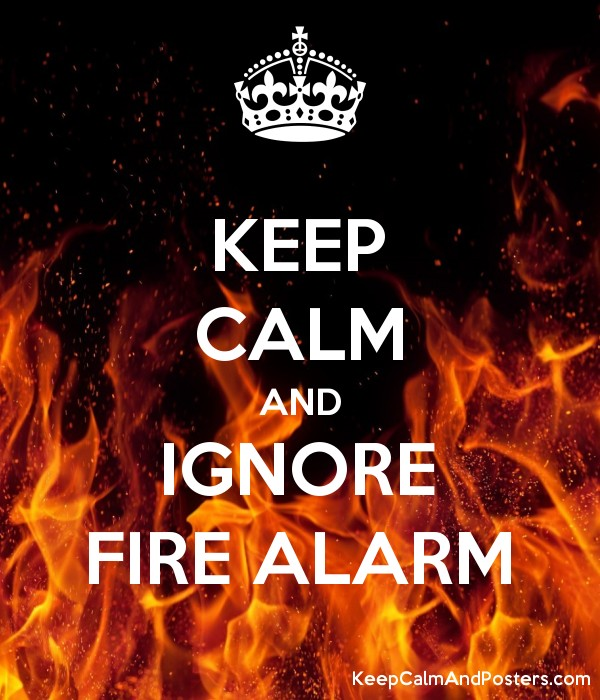
\includegraphics[width=0.3\textwidth]{images/ignorefirealarm.jpg}
	\end{center}


\end{frame}

\begin{frame}
	\frametitle{Disabling Interrupts}

	While interrupts are disabled, the system will be unable to respond to user input or other events (e.g., a fire alarm or detection of an incoming missile!).

	\begin{center}
		
\includegraphics[width=\textwidth]{images/thisisfine.png}
	\end{center}

	If an error is encountered in the critical section and the program is terminated, the system is effectively stuck because no other program will be able to run.


\end{frame}

\begin{frame}
	\frametitle{Disabling Interrupts}

	If we have multiple processors the disabling interrupts will not be sufficient.

	But maybe we're on the right track by getting hardware involved.


	The hardware designers were aware of the problem and have kindly provided a facility to help us out: the \alert{Test-and-Set} instruction.


\end{frame}

\begin{frame}[fragile]
	\frametitle{Test-and-Set}

	The Test-and-Set instruction is a special machine instruction that is performed in a single instruction cycle and is therefore not interruptible.

	It is therefore an atomic read and write.

	Its semantics in C are:

	\begin{verbatim}
boolean test_and_set( int* i ) {
  if ( *i == 0 ) {
    *i = 1;
    return true;
  } else {
    return false;
  }
}
\end{verbatim}

\end{frame}

\begin{frame}[fragile]
	\frametitle{Test-and-Set}

	Now let us put it into action.

	\begin{verbatim}
while ( !test_and_set( busy ) ) {
   /* Wait for my turn */
}
/* critical section */
busy = 0;
\end{verbatim}


	(Both $A$ and $B$ would be the same, so only one copy is shown)


\end{frame}

\begin{frame}
	\frametitle{Mutual Exclusion Success!}

	Finally, we have something that will provide mutual exclusion without the risk that the threads will all get stuck because each thinks another is in the critical section.

	This is good, but can be improved.

	The \texttt{while} loop that is constantly checking the value with the Test-and-Set instruction is an example of \alert{busy-waiting}.

	A given thread is constantly checking and checking and checking the instruction, and this is a waste of time and effort.

\end{frame}

\begin{frame}
	\frametitle{Busy-Waiting}

	It is less wasteful of resources and effort if the \texttt{while} loop contains some instructions saying it should wait a little while before checking again.

	Serialization was achievable through messages; and they can be used to get mutual exclusion. This is the topic to be examined next.


\end{frame}

\end{document}

